\documentclass[12pt,a4paper]{report}
\usepackage[a4paper,margin=1in]{geometry}
\usepackage{graphicx, tikz, float, array, booktabs, longtable, amsmath, setspace, titlesec, hyperref}
\usetikzlibrary{arrows.meta,positioning,shapes.geometric,shapes.misc,calc}
\hypersetup{hidelinks}
\setstretch{1.15}
\newcommand{\CourseHeader}{UCS503 -- Software Engineering}
\newcommand{\ProjectName}{SmartCross}
\newcommand{\ProjectSubtitle}{Real-Time Railway Crossing Safety and Prediction System}
\newcommand{\StudentDetails}{\texttt{1024030925} Moksh\\\texttt{1024030312} Sandeep Yadav\\\texttt{1024030314} Gagandeep Singh}
\newcommand{\GroupDetails}{Group: \texttt{2C23} \quad B.E. Third Year, CSE}
\newcommand{\AdvisorDetails}{Dr. Jhonsy Bansal}
\tikzset{blk/.style={draw,rounded corners,align=center,minimum width=2.5cm,minimum height=.8cm,font=\small,fill=blue!5},
arr/.style={-{Latex[length=2mm]},thick}}
\begin{document}
\begin{titlepage}\centering\vspace*{1.5cm}
{\Large\bfseries \CourseHeader\par}\vspace{2cm}
{\Huge\bfseries \ProjectName\par}\vspace{.6cm}
{\Large \ProjectSubtitle\par}\vspace{2cm}
{\large \StudentDetails\par}\vspace{1cm}
{\large \GroupDetails\par}\vspace{1cm}
{\large\bfseries Faculty Advisor\par}{\large \AdvisorDetails\par}
\vfill{\Large\bfseries End-Semester Evaluation Report\par}\vspace{.4cm}
Department of Computer Science and Engineering\\Thapar Institute of Engineering and Technology, Patiala
\end{titlepage}
\tableofcontents
\chapter*{Abstract}\addcontentsline{toc}{chapter}{Abstract}
SmartCross is a web-based railway-crossing monitoring and prediction system developed for four level crossings on the Patiala (PTA)--Dhablan (DBN) corridor: Phatak 19, 20, 23 and 24. It combines train timetable information, live train observations from the RailRadar API, OpenStreetMap-derived railway geometry and historical observations to estimate train arrival and crossing-impact windows. The system presents predicted crossing states, estimated waiting information, train direction, prediction source and confidence through a React interface. A Node.js/Express backend coordinates data acquisition, prediction, persistence and real-time delivery through Socket.IO, while MongoDB stores operational and historical records. A simulation mode exercises the same processing pipeline when live API access is unavailable. SmartCross has no physical gate sensors; all displayed crossing states are software predictions and must not be interpreted as direct confirmation of barrier position.
\chapter{1. Introduction}
Railway level crossings create an interaction point between road traffic and railway traffic. Road users may have limited information about an approaching train, the likely start of a closure, or the estimated time until the crossing becomes available. A train-tracking application may show a train's location but does not necessarily translate that information into a crossing-specific advisory.

SmartCross addresses this information gap by relating train movement to a defined railway corridor and its crossings. The initial implementation focuses on the Patiala--Dhablan corridor in Punjab, India, and monitors four crossings: 19, 20, 23 and 24. It estimates the effect of monitored passenger trains on each crossing and communicates the result through a browser-based dashboard, map, train views, alerts and analytics.

\section{Problem Statement}
To design and implement a software system that consumes available train timetable and live-status data, maps train progress onto a railway corridor, estimates arrival and clearance windows at selected level crossings, and communicates predicted crossing conditions to road users in a timely and understandable manner. The system must handle missing, delayed or inconsistent input data without presenting unsupported certainty.

\section{Objectives}
\begin{itemize}\item 1. Integrate an external train-data provider and normalize its responses.\end{itemize}
\begin{itemize}\item 2. Represent the railway corridor and crossing locations using geographic data and along-track distance.\end{itemize}
\begin{itemize}\item 3. Estimate train arrival times using live observations and controlled fallback sources.\end{itemize}
\begin{itemize}\item 4. Derive crossing advisories through a state machine that considers multiple trains and direction of travel.\end{itemize}
\begin{itemize}\item 5. Provide live dashboard updates, map views, alerts, train details and operational analytics.\end{itemize}
\begin{itemize}\item 6. Provide a simulation environment for development and demonstration when live data is unavailable.\end{itemize}
7. Persist train observations, predictions, crossing events, alerts and administrative audit information.

\section{Scope and Safety Boundary}
The implemented corridor contains Phatak 19 (Station Approach), 20 (Sirhind Road), 23 (Model Town Extension) and 24 (Dhablan Approach). The crossings are arranged into Group A (19 and 20) and Group B (23 and 24). The project monitors configured passenger trains; unscheduled trains and freight trains are not covered by the current prediction scope.

SmartCross does not use physical gate-position sensors. A status such as CLOSED is a prediction derived from train position and configured software thresholds, not a sensor reading or railway-authority confirmation. Timetable-only and historical-only estimates are not permitted to assert CLOSED. The interface and report must preserve this distinction.

\chapter{2. System Analysis and Requirements}
\subsection{2.1 Functional requirements}
\begin{itemize}\item FR-01: Retrieve live status for configured trains when live mode is enabled.\end{itemize}
\begin{itemize}\item FR-02: Normalize and validate provider data; retain a mock provider for simulation.\end{itemize}
\begin{itemize}\item FR-03: Resolve train progress to a chainage position on the railway corridor.\end{itemize}
\begin{itemize}\item FR-04: Estimate per-crossing arrival, closure-start and reopening windows.\end{itemize}
\begin{itemize}\item FR-05: Determine OPEN, CLOSING\_SOON, CLOSED, OPENING\_SOON or UNKNOWN advisories.\end{itemize}
\begin{itemize}\item FR-06: Account for train direction, multiple trains and grouped crossing impacts.\end{itemize}
\begin{itemize}\item FR-07: Expose corridor state, crossings, trains, predictions, alerts and analytics through REST endpoints.\end{itemize}
\begin{itemize}\item FR-08: Push snapshots and status changes to connected clients using Socket.IO.\end{itemize}
\begin{itemize}\item FR-09: Allow authenticated administrators to manage settings, modes and simulation controls.\end{itemize}
\begin{itemize}\item FR-10: Store operational observations, prediction samples, events and audit records in MongoDB.\end{itemize}
\subsection{2.2 Non-functional requirements}
\begin{itemize}\item Performance: updates and API responses should be suitable for near-real-time use, subject to provider latency and quota.\end{itemize}
\begin{itemize}\item Reliability: bounded retries, caching, stale-data checks, fallback prediction and UNKNOWN state reduce the risk of presenting invalid data as current.\end{itemize}
\begin{itemize}\item Scalability: corridor configuration and services are modular, allowing additional crossings and monitored trains to be configured.\end{itemize}
\begin{itemize}\item Usability: crossing states, train details, confidence and source information are presented in dedicated interface views.\end{itemize}
\begin{itemize}\item Security: administrator operations use password-based authentication and JWTs; the backend includes request validation, rate limiting, security headers and controlled CORS.\end{itemize}
\begin{itemize}\item Maintainability: the backend separates controllers, services, models, middleware and configuration; the frontend separates pages, components, contexts and API utilities.\end{itemize}
\chapter{3. System Architecture and Design}
SmartCross uses a client--server architecture. External train information is obtained by the RailRadar client and passed through normalization and position resolution. The corridor engine invokes the prediction and gate-state services, stores resulting records and emits snapshots and events. The React frontend consumes REST data for initial and recovery synchronization and Socket.IO for updates.

\subsection{3.1 Backend modules}
RailRadar client: performs bounded requests, timeout and retry handling, response caching, in-flight request de-duplication and quota-header tracking.

Normalizer and position resolver: converts provider payloads into a consistent observation and maps route progress to corridor chainage. The documented live response does not provide train latitude/longitude; route kilometre information is used to resolve position. An undocumented coordinate is accepted only if it lies within 300 m of the track.

Corridor engine: coordinates observations, prediction, state aggregation, persistence and event emission.

Prediction services: calculate effective speed and ETA, select a fallback source, smooth noisy ETA changes, and evaluate historical prediction error.

Gate services: apply crossing-state transitions, multiple-train precedence and hysteresis; grouped-closure logic reports the sequence and overlap of crossings in each group.

Scheduler and simulation: the adaptive scheduler determines when and how frequently trains are polled; the simulation engine feeds mock RailRadar-format observations through the same normalization and prediction pipeline.

Alert, analytics and WebSocket services: generate deduplicated alerts, summarize recorded and predicted metrics, and deliver real-time events.

\chapter{3.2 Frontend Modules}
The React frontend uses Vite, React Router, Leaflet/React-Leaflet, Recharts and Socket.IO Client. Its implemented pages include Dashboard, Map, Trains, Train Detail, Crossing Detail, Alerts, Analytics, Admin, Settings and Simulation. Shared components include the application layout, crossing cards, countdown display and corridor map. Live-data, authentication and notification contexts coordinate state and user-facing updates.

\chapter{3.3 Architecture Diagram}
\begin{figure}[H]\centering
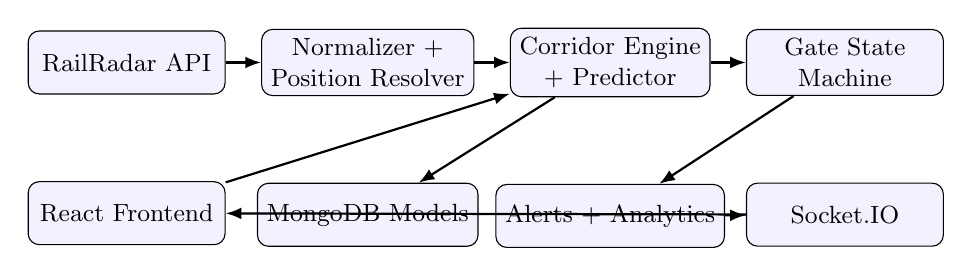
\begin{tikzpicture}[node distance=0.7cm and 0.45cm]
\node[blk] (rr) {RailRadar API};
\node[blk,right=of rr] (norm) {Normalizer +\\ Position Resolver};
\node[blk,right=of norm] (eng) {Corridor Engine\\ + Predictor};
\node[blk,right=of eng] (gate) {Gate State\\ Machine};
\node[blk,below=1.1cm of norm] (db) {MongoDB Models};
\node[blk,below=1.1cm of eng] (svc) {Alerts + Analytics};
\node[blk,below=1.1cm of gate] (ws) {Socket.IO};
\node[blk,below=1.1cm of rr] (fe) {React Frontend};
\draw[arr] (rr)--(norm);\draw[arr] (norm)--(eng);\draw[arr] (eng)--(gate);
\draw[arr] (eng)--(db);\draw[arr] (gate)--(svc);\draw[arr] (svc)--(ws);
\draw[arr] (ws)--(fe);\draw[arr] (fe)--(eng);
\end{tikzpicture}\caption{High-level SmartCross architecture}\end{figure}
\chapter{4. Corridor and Geographic Model}
The corridor is represented using an OpenStreetMap-derived track polyline. Linear referencing converts a geographic observation into chainage, measured in metres from Patiala station, increasing towards Dhablan. This is more suitable than straight-line GPS distance because trains follow the railway alignment.

Crossing reference data in the project configuration:

\begin{itemize}\item Phatak 19 --- Station Approach --- chainage approximately 427 m from Patiala.\end{itemize}
\begin{itemize}\item Phatak 20 --- Sirhind Road --- chainage approximately 1,001 m.\end{itemize}
\begin{itemize}\item Phatak 23 --- Model Town Extension --- chainage approximately 3,508 m.\end{itemize}
\begin{itemize}\item Phatak 24 --- Dhablan Approach --- chainage approximately 4,449 m.\end{itemize}
Dhablan station is represented at approximately 11,957 m along the corridor. The supplied project documentation reports that the four crossing coordinates are within approximately 1--3 m of nodes on the OSM railway line. The exact Dhablan platform position is not independently confirmed and regional extensions are coarse display/dead-reckoning bounds.

Group A contains crossings 19 and 20; Group B contains crossings 23 and 24. A grouped advisory does not assume that two barriers close simultaneously: each crossing retains its own predicted closure window and overlap flag.

\chapter{5. Prediction Methodology}
\subsection{5.1 Chainage and direction}
Let s\_train be the train's chainage, s\_crossing the crossing chainage, and d the direction sign (+1 from Patiala to Dhablan, -1 from Dhablan to Patiala). The along-track distance ahead is:

\[\mathrm{distance}_{ahead}=(s_{crossing}-s_{train})\times d\]
\subsection{5.2 ETA}
ETA is estimated as distance ahead divided by effective speed. Effective speed blends measured speed (70\%) with recent observed speeds (30\%), and falls back to historical average and then a configured default. The value is clamped to configured minimum and maximum speeds. A stopped train at a terminal station accounts for remaining scheduled dwell; a stopped train between stations receives a restart allowance. Predictions beyond six hours are treated as UNKNOWN.

\subsection{5.3 Five-level fallback strategy}
\begin{itemize}\item Level 1 --- LIVE\_POSITION: fresh positional observation (up to the configured 180-second stale threshold); normally highest confidence.\end{itemize}
\begin{itemize}\item Level 2 --- LATEST\_OBSERVATION: dead reckoning from a recent observation (up to 900 seconds), with stop/dwell handling.\end{itemize}
\begin{itemize}\item Level 3 --- TIMETABLE\_WITH\_DELAY: timetable estimate adjusted using a sufficiently recent observed delay.\end{itemize}
\begin{itemize}\item Level 4 --- HISTORICAL\_AVERAGE: historical offset from scheduled corridor entry, requiring at least five observed live passages.\end{itemize}
\begin{itemize}\item Level 5 --- TIMETABLE\_ESTIMATE: timetable-only interpolation along the corridor; low confidence.\end{itemize}
If no valid source exists, the prediction is UNKNOWN. Confidence is reduced for long prediction horizons. Each prediction records its source, level, confidence, train, calculation time, predicted arrival, ETA, closure start, reopening time and estimated closure duration.

\subsection{5.4 Smoothing and outlier handling}
ETA values are smoothed against expected countdown decay. A single change exceeding 120 seconds is treated as an outlier and only partially applied; persistent changes can subsequently be accepted. Position changes implying more than 1.5 times the configured maximum train speed are rejected. Repeated movement opposite to the expected direction can update the inferred direction.

\subsection{5.5 Closure-window estimation}
Closure start is estimated from configured distance and ETA thresholds. Reopening is estimated after the train tail has passed a clearance distance and buffer. Train length, clearance distance and buffer are software parameters, not measured physical barrier timings.

\section{Prediction Flow Diagram}
\begin{figure}[H]\centering
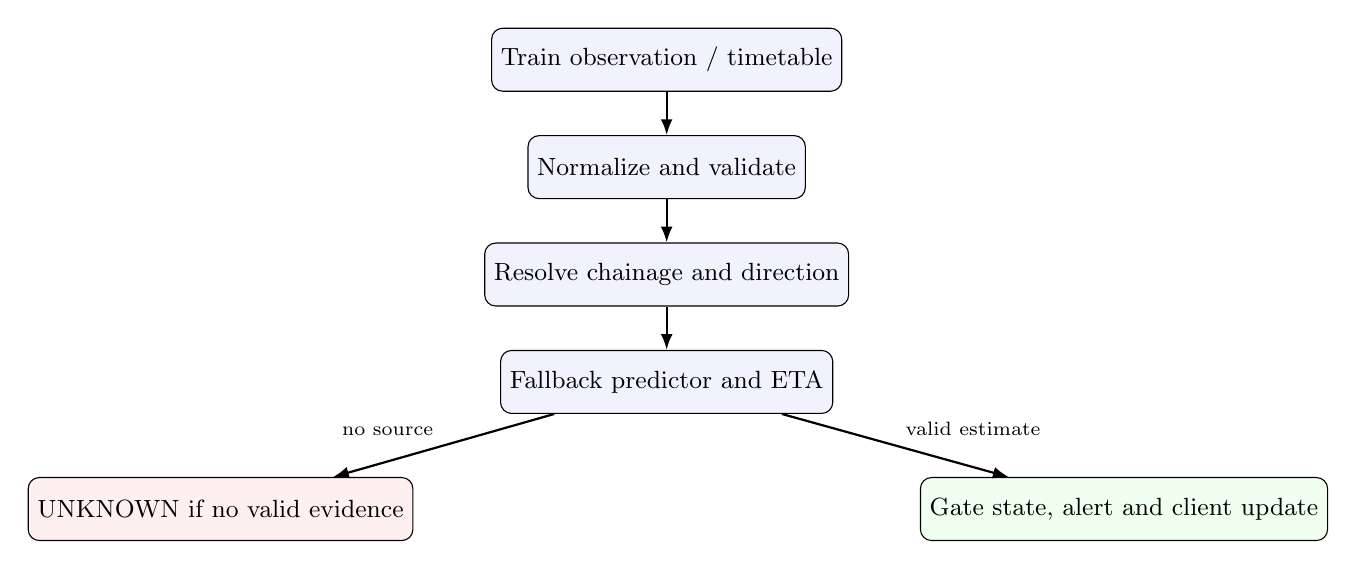
\begin{tikzpicture}[node distance=.55cm]
\node[blk] (a) {Train observation / timetable};
\node[blk,below=of a] (b) {Normalize and validate};
\node[blk,below=of b] (c) {Resolve chainage and direction};
\node[blk,below=of c] (d) {Fallback predictor and ETA};
\node[blk,below left=0.8cm and 1.1cm of d,fill=red!6] (u) {UNKNOWN if no valid evidence};
\node[blk,below right=0.8cm and 1.1cm of d,fill=green!6] (g) {Gate state, alert and client update};
\draw[arr] (a)--(b);\draw[arr] (b)--(c);\draw[arr] (c)--(d);\draw[arr] (d)--node[above left,font=\scriptsize]{no source}(u);\draw[arr] (d)--node[above right,font=\scriptsize]{valid estimate}(g);
\end{tikzpicture}\caption{Train-to-crossing prediction flow}\end{figure}
\chapter{6. Crossing State Machine and Grouped Closures}
The state machine uses OPEN, CLOSING\_SOON, CLOSED, OPENING\_SOON and UNKNOWN. The configured CLOSING\_SOON threshold is 10 minutes. CLOSED is predicted when positional evidence places a moving train within the configured 1,200 m distance or 2.5-minute ETA threshold, or when the train occupies the crossing. OPENING\_SOON represents a train whose head has passed but whose tail/clearance window is not yet complete. OPEN requires clearance and no other train within the warning window.

Safety-oriented precedence for multiple trains is CLOSED, OPENING\_SOON, CLOSING\_SOON, UNKNOWN, then OPEN. Thus, one train passing cannot make a crossing OPEN if another train is approaching. Timetable/historical estimates can at most produce CLOSING\_SOON and never assert CLOSED. Escalations and passage-driven transitions are immediate; other downgrades require a configured confirmation interval (hysteresis) to reduce status flicker.

Grouped closure detection operates on Group A (19/20) and Group B (23/24), reporting the order in which crossings are affected and whether their individual predicted windows overlap. It does not infer simultaneous barrier operation.

\chapter{7. Adaptive Polling and Data Acquisition}
The timetable controls when live polling begins: polling is scheduled from 20 minutes before a train's corridor entry until 10 minutes after corridor exit/clearance. Proximity controls polling frequency: the configured near, middle and far intervals are 45, 90 and 180 seconds respectively. The scheduler also considers the remaining monthly quota and a daily budget. RailRadar response quota headers are tracked where available.

The RailRadar client accesses the live endpoint for configured train numbers. The schedule endpoint can be refreshed when enabled, but the bundled timetable is available as a local source. When the API key is absent, AUTO mode selects simulation rather than representing mock data as live data. Live and simulation records are mode-tagged and engine state is reset when switching modes.

\chapter{8. Simulation, Alerts and Analytics}
The simulation module supports multiple trains, direction, speed, delay, pause/resume, signal loss, train removal and scenario-based runs. Simulated trains are labelled SIM and the interface displays a persistent simulation indicator. Simulation observations pass through a mock provider that returns RailRadar-shaped payloads, allowing the normalizer, resolver, predictor and state machine to be exercised consistently.

Alerts include crossing status changes and are deduplicated. The frontend supports in-app notifications, audio, browser notifications, configurable warning threshold, mute/volume controls and alert history. Analytics include train frequency and speed, estimated waiting time, predicted-versus-observed arrival error, error by horizon/source, closure patterns, source distribution and API usage. Charts distinguish RECORDED, PREDICTED and ESTIMATED data and can separate live from simulated records.

\chapter{9. Database Design}
MongoDB is accessed through Mongoose. The project defines models for Phatak, Train, TrainSchedule, TrainRoute, TrainLiveSnapshot, TrainPhatakMapping, PhatakPrediction, Prediction, PredictionEvaluation, HistoricalTrainObservation, GateEvent, Alert, NotificationSubscription, SystemSetting and AuditLog.

\begin{itemize}\item Phatak stores crossing reference and last predicted state; Train and TrainSchedule store monitored train and timetable information; TrainLiveSnapshot stores deduplicated live observations; TrainPhatakMapping stores train/crossing sequences; PhatakPrediction stores current per-mode predictions; Prediction and PredictionEvaluation support horizon-based evaluation; HistoricalTrainObservation stores positional passages; GateEvent stores state transitions; Alert stores deduplicated alerts; NotificationSubscription stores browser preferences; SystemSetting stores runtime thresholds and monitored train configuration; AuditLog records API calls and administrative actions.\end{itemize}
Indexes enforce uniqueness for key identities and support geospatial lookup, time-based queries and TTL retention. Documented retention includes 14 days for snapshots, 60 days for audit records, 90 days for alerts and 365 days for events; prediction records have their own short TTL policies.

\section{Data Model Diagram}
\begin{figure}[H]\centering
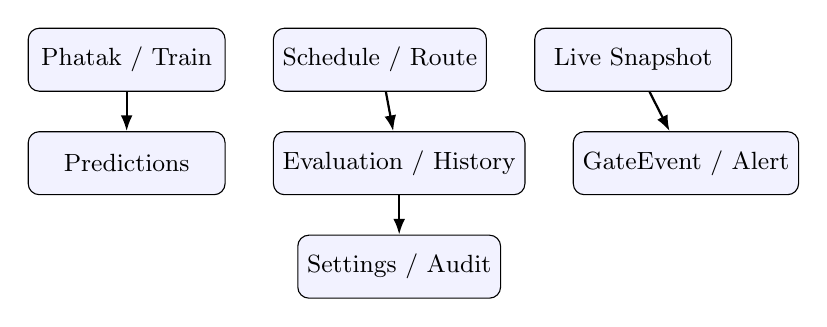
\begin{tikzpicture}[node distance=.5cm and .6cm]
\node[blk] (a) {Phatak / Train};
\node[blk,right=of a] (b) {Schedule / Route};
\node[blk,right=of b] (c) {Live Snapshot};
\node[blk,below=of a] (d) {Predictions};
\node[blk,right=of d] (e) {Evaluation / History};
\node[blk,right=of e] (f) {GateEvent / Alert};
\node[blk,below=of e] (g) {Settings / Audit};
\draw[arr] (a)--(d);\draw[arr] (b)--(e);\draw[arr] (c)--(f);\draw[arr] (e)--(g);
\end{tikzpicture}\caption{Logical database grouping}\end{figure}
\chapter{10. API and Real-Time Communication}
The backend exposes a REST API under /api. Public endpoints include /health, /state, /corridor, /system/status, /phataks, /trains, /predictions, /alerts, /analytics/summary, /settings and /simulation/status. Administrative endpoints include authentication, settings changes, mode changes, operational metrics/logs, prediction recalculation, train refresh and simulation controls.

Socket.IO events include corridor:snapshot, train:update, phatak:update, gate:status-change, alert:new and system:status. Snapshots carry increasing sequence numbers; clients discard duplicate or out-of-order events and can request a snapshot. On reconnection, the frontend can resynchronize through REST.

\chapter{11. Security and Operational Controls}
The backend uses Helmet security headers, configured CORS, rate limiting, request validation, centralized error handling and JWT-protected administrative routes. The admin login endpoint is rate-limited. Environment variables hold the administrator password, JWT secret, database URI and optional RailRadar API key; real secrets must not be committed to source control. Production configuration requires explicit database and secret configuration, while in-memory MongoDB is intended for development/testing only.

These controls reduce common application risks but do not establish that the application is production-certified or immune to attack. Deployment should use HTTPS, strong unique secrets, restricted database network access, regular dependency updates, backups, monitoring and a security review. Access control and operational procedures should be tested before public deployment.

\chapter{12. Testing and Evaluation}
The project repository contains 13 Jest test suites covering GIS and position resolution, ETA, smoothing, fallback prediction, gate-state transitions, grouped closures, engine behaviour, RailRadar client and normalization, scheduler, simulation, REST API and Socket.IO integration. The project README records a verification run of 13 suites and 132 tests passing. This is a repository-reported result; it is not a new test execution performed for this report.

Additional checks recorded in the project README include frontend production build, desktop/mobile UI exercise in headless Chrome, local fake-RailRadar integration and production startup checks. The README notes that real RailRadar responses could not be verified in that build environment because the API host was unreachable, and Docker Compose execution could not be performed because a Docker daemon was unavailable (configuration validation was performed).

Evaluation should measure: (i) train-data normalization success, (ii) crossing identification and chainage resolution, (iii) ETA error by prediction horizon, (iv) state-transition correctness, (v) alert delivery latency, (vi) REST and Socket.IO responsiveness, (vii) API quota consumption and (viii) behaviour under stale or missing data. No numeric live-world accuracy or availability percentage is claimed because verified field measurements are not included in the supplied project materials.

\section{Test Coverage Matrix}
\begin{longtable}{p{.22\textwidth}p{.34\textwidth}p{.34\textwidth}}
\toprule Area & Test focus & Evidence in repository\\
\midrule
GIS / corridor & Coordinate helpers, chainage, position resolution & gis.test.js\\
Prediction & ETA, fallback levels, smoothing & eta.test.js; fallbackPredictor.test.js; smoother.test.js\\
State logic & Thresholds, multiple trains, hysteresis & gateStateMachine.test.js\\
Grouped closures & Sequence and overlap & groupedClosure.test.js\\
Data provider & Normalization, client retry/quota behaviour & normalizer.test.js; railRadarClient.test.js\\
Scheduler / simulation & Polling plan and scenario behaviour & scheduler.test.js; simulation.test.js\\
Integration & REST endpoints, admin protection, sockets & api.integration.test.js; socket.integration.test.js\\
\bottomrule
\end{longtable}
\chapter{13. Limitations and Future Work}
\subsection{Current limitations}
\begin{itemize}\item 1. No physical gate sensors are integrated; status is predicted rather than measured.\end{itemize}
\begin{itemize}\item 2. Only configured passenger trains are monitored; freight and unscheduled trains are outside the current scope.\end{itemize}
\begin{itemize}\item 3. Real live API behaviour depends on provider availability, credentials, quota and response quality.\end{itemize}
\begin{itemize}\item 4. Historical prediction quality depends on collecting enough verified live passage observations.\end{itemize}
\begin{itemize}\item 5. Regional track extensions are coarse; the Dhablan station platform point requires independent verification.\end{itemize}
\begin{itemize}\item 6. The supplied materials do not include a field trial dataset proving real-world prediction accuracy or safety impact.\end{itemize}
\subsection{Future work}
\begin{itemize}\item 1. Conduct supervised field validation and compare predicted events with manually verified crossing observations.\end{itemize}
\begin{itemize}\item 2. Investigate an authoritative gate-state feed or sensor integration, with source provenance and fail-safe handling.\end{itemize}
\begin{itemize}\item 3. Expand train coverage only after validating data availability and route mapping for each additional service.\end{itemize}
\begin{itemize}\item 4. Improve historical learning with more observations and report error distributions by horizon and direction.\end{itemize}
\begin{itemize}\item 5. Perform load, resilience, security and deployment testing in a controlled environment.\end{itemize}
\begin{itemize}\item 6. Improve operational monitoring for API quota, stale data, missed polls and service health.\end{itemize}
\chapter{14. Conclusion}
SmartCross has progressed from the initial concept documented in the Mid-Semester Evaluation to a modular implementation focused on the Patiala--Dhablan railway corridor. The supplied project includes a React frontend, Node.js/Express backend, MongoDB models, RailRadar integration, OSM-based corridor geometry, a multi-level prediction strategy, crossing state machine, adaptive polling, simulation, alerts, analytics, REST endpoints and Socket.IO updates.

The most important design principle is to communicate both the predicted crossing condition and the evidence behind it. By retaining source and confidence information, separating live and simulated modes, and using UNKNOWN when evidence is insufficient, the system avoids presenting every estimate as certainty. Further field validation and authoritative crossing-state integration are necessary before the system can be treated as a safety-critical operational service.

\chapter{References}
\begin{itemize}\item 1. SmartCross v2 project source code and README supplied for this evaluation (uploaded archive smartcross-v2.zip).\end{itemize}
\begin{itemize}\item 2. SmartCross Mid-Semester Evaluation report supplied by the project team.\end{itemize}
\begin{itemize}\item 3. RailRadar API documentation referenced by the project README: https://railradar.in/docs.\end{itemize}
\begin{itemize}\item 4. OpenStreetMap railway geometry, as incorporated into the supplied project data. OpenStreetMap data is distributed under the Open Database License (ODbL).\end{itemize}

\chapter{References}
\begin{enumerate}
\item SmartCross v2 project source code and README supplied for this evaluation (uploaded archive \texttt{smartcross-v2.zip}).
\item SmartCross Mid-Semester Evaluation report supplied by the project team.
\item RailRadar API documentation referenced by the project README: \url{https://railradar.in/docs}.
\item OpenStreetMap railway geometry incorporated into the supplied project data; OpenStreetMap data is distributed under the Open Database License (ODbL).
\end{enumerate}
\end{document}
